\section{eo\-Parse\-Tree$<$ FType, Node $>$ Class Template Reference}
\label{classeo_parse_tree}\index{eoParseTree@{eoParseTree}}
Implementation of parse-tree for genetic programming.  


{\tt \#include $<$gp/eo\-Parse\-Tree.h$>$}

Inheritance diagram for eo\-Parse\-Tree$<$ FType, Node $>$::\begin{figure}[H]
\begin{center}
\leavevmode
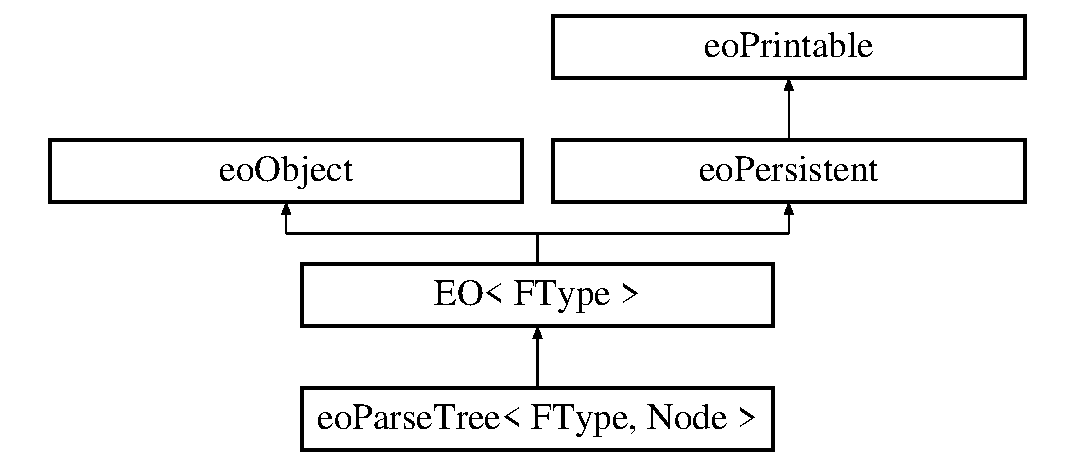
\includegraphics[height=4cm]{classeo_parse_tree}
\end{center}
\end{figure}
\subsection*{Public Types}
\begin{CompactItemize}
\item 
typedef parse\_\-tree$<$ Node $>$::subtree {\bf Subtree}\label{classeo_parse_tree_w0}

\item 
typedef Node {\bf reference}\label{classeo_parse_tree_w1}

\item 
typedef const reference {\bf const\_\-reference}\label{classeo_parse_tree_w2}

\end{CompactItemize}
\subsection*{Public Member Functions}
\begin{CompactItemize}
\item 
{\bf eo\-Parse\-Tree} (void)\label{classeo_parse_tree_a0}

\begin{CompactList}\small\item\em Default Constructor. \item\end{CompactList}\item 
{\bf eo\-Parse\-Tree} (const parse\_\-tree$<$ Node $>$ \&tree)
\begin{CompactList}\small\item\em Copy Constructor. \item\end{CompactList}\item 
virtual void {\bf prune\-Tree} (unsigned \_\-size)
\begin{CompactList}\small\item\em To prune me to a certain size. \item\end{CompactList}\item 
{\bf eo\-Parse\-Tree} (std::istream \&is)
\begin{CompactList}\small\item\em To read me from a stream. \item\end{CompactList}\item 
std::string {\bf class\-Name} (void) const \label{classeo_parse_tree_a4}

\begin{CompactList}\small\item\em My class name. \item\end{CompactList}\item 
void {\bf print\-On} (std::ostream \&os) const 
\begin{CompactList}\small\item\em To print me on a stream. \item\end{CompactList}\item 
void {\bf read\-From} (std::istream \&is)
\begin{CompactList}\small\item\em To read me from a stream. \item\end{CompactList}\end{CompactItemize}


\subsection{Detailed Description}
\subsubsection*{template$<$class FType, class Node$>$ class eo\-Parse\-Tree$<$ FType, Node $>$}

Implementation of parse-tree for genetic programming. 



Definition at line 54 of file eo\-Parse\-Tree.h.

\subsection{Constructor \& Destructor Documentation}
\index{eoParseTree@{eo\-Parse\-Tree}!eoParseTree@{eoParseTree}}
\index{eoParseTree@{eoParseTree}!eoParseTree@{eo\-Parse\-Tree}}
\subsubsection{\setlength{\rightskip}{0pt plus 5cm}template$<$class FType, class Node$>$ {\bf eo\-Parse\-Tree}$<$ FType, Node $>$::{\bf eo\-Parse\-Tree} (const parse\_\-tree$<$ Node $>$ \& {\em tree})\hspace{0.3cm}{\tt  [inline]}}\label{classeo_parse_tree_a1}


Copy Constructor. 

\begin{Desc}
\item[Parameters:]
\begin{description}
\item[{\em tree}]The tree to copy \end{description}
\end{Desc}


Definition at line 79 of file eo\-Parse\-Tree.h.\index{eoParseTree@{eo\-Parse\-Tree}!eoParseTree@{eoParseTree}}
\index{eoParseTree@{eoParseTree}!eoParseTree@{eo\-Parse\-Tree}}
\subsubsection{\setlength{\rightskip}{0pt plus 5cm}template$<$class FType, class Node$>$ {\bf eo\-Parse\-Tree}$<$ FType, Node $>$::{\bf eo\-Parse\-Tree} (std::istream \& {\em is})\hspace{0.3cm}{\tt  [inline]}}\label{classeo_parse_tree_a3}


To read me from a stream. 

\begin{Desc}
\item[Parameters:]
\begin{description}
\item[{\em is}]The std::istream \end{description}
\end{Desc}


Definition at line 102 of file eo\-Parse\-Tree.h.

References eo\-Parse\-Tree$<$ FType, Node $>$::read\-From().

\subsection{Member Function Documentation}
\index{eoParseTree@{eo\-Parse\-Tree}!pruneTree@{pruneTree}}
\index{pruneTree@{pruneTree}!eoParseTree@{eo\-Parse\-Tree}}
\subsubsection{\setlength{\rightskip}{0pt plus 5cm}template$<$class FType, class Node$>$ virtual void {\bf eo\-Parse\-Tree}$<$ FType, Node $>$::prune\-Tree (unsigned {\em \_\-size})\hspace{0.3cm}{\tt  [inline, virtual]}}\label{classeo_parse_tree_a2}


To prune me to a certain size. 

\begin{Desc}
\item[Parameters:]
\begin{description}
\item[{\em \_\-size}]My maximum size \end{description}
\end{Desc}


Definition at line 86 of file eo\-Parse\-Tree.h.

Referenced by eo\-Collapse\-Subtree\-Mutation$<$ FType, Node $>$::operator()(), eo\-Expansion\-Mutation$<$ FType, Node $>$::operator()(), eo\-Branch\-Mutation$<$ FType, Node $>$::operator()(), and eo\-Subtree\-XOver$<$ FType, Node $>$::operator()().\index{eoParseTree@{eo\-Parse\-Tree}!printOn@{printOn}}
\index{printOn@{printOn}!eoParseTree@{eo\-Parse\-Tree}}
\subsubsection{\setlength{\rightskip}{0pt plus 5cm}template$<$class FType, class Node$>$ void {\bf eo\-Parse\-Tree}$<$ FType, Node $>$::print\-On (std::ostream \& {\em os}) const\hspace{0.3cm}{\tt  [inline, virtual]}}\label{classeo_parse_tree_a5}


To print me on a stream. 

\begin{Desc}
\item[Parameters:]
\begin{description}
\item[{\em os}]The std::ostream \end{description}
\end{Desc}


Reimplemented from {\bf EO$<$ FType $>$} {\rm (p.\,\pageref{class_e_o_z10_2})}.

Definition at line 114 of file eo\-Parse\-Tree.h.

References EO$<$ F $>$::print\-On().\index{eoParseTree@{eo\-Parse\-Tree}!readFrom@{readFrom}}
\index{readFrom@{readFrom}!eoParseTree@{eo\-Parse\-Tree}}
\subsubsection{\setlength{\rightskip}{0pt plus 5cm}template$<$class FType, class Node$>$ void {\bf eo\-Parse\-Tree}$<$ FType, Node $>$::read\-From (std::istream \& {\em is})\hspace{0.3cm}{\tt  [inline, virtual]}}\label{classeo_parse_tree_a6}


To read me from a stream. 

\begin{Desc}
\item[Parameters:]
\begin{description}
\item[{\em is}]The std::istream \end{description}
\end{Desc}


Reimplemented from {\bf EO$<$ FType $>$} {\rm (p.\,\pageref{class_e_o_z10_1})}.

Definition at line 128 of file eo\-Parse\-Tree.h.

References EO$<$ F $>$::read\-From().

Referenced by eo\-Parse\-Tree$<$ FType, Node $>$::eo\-Parse\-Tree().

The documentation for this class was generated from the following file:\begin{CompactItemize}
\item 
eo\-Parse\-Tree.h\end{CompactItemize}
